\documentclass[a4paper,12pt]{article}
\usepackage[T1]{fontenc}
\usepackage[utf8]{inputenc}
\usepackage{lmodern}
\usepackage{CJKutf8}
\usepackage{indentfirst}
\usepackage{graphicx}
\usepackage{enumerate}
\usepackage{float}
\usepackage{tabularx}
\usepackage{fancyhdr}
\usepackage{times}
\usepackage{caption}
\usepackage{afterpage}
%\usepackage{titlesec}
\usepackage[pdftex, 
pdfstartview=FitH, unicode=true, bookmarksnumbered=true,
bookmarksopen=true, colorlinks=false,
pdfborder={1 0 0}, citecolor=black ]{hyperref}

\setlength{\parindent}{2em}
\addtolength{\textwidth}{4.0cm}
\addtolength{\textheight}{2.0cm}
\addtolength{\voffset}{-2cm}
\addtolength{\hoffset}{-1.5cm}

\renewcommand\contentsname{目录}
\renewcommand\figurename{图}
\renewcommand\tablename{表}
\renewcommand\refname{参考文献}

\newcolumntype{Y}{>{\centering\arraybackslash}X}

\setcounter{secnumdepth}{5}

\makeatletter
\renewcommand\paragraph{\@startsection{paragraph}{4}{\z@}%
{3.25ex \@plus1ex \@minus.2ex}%
{1.5ex \@plus.2ex}%
{\normalfont\normalsize\bfseries}}
\makeatother

\makeatletter
\renewcommand\subparagraph{\@startsection{subparagraph}{5}{\z@}%
{3.25ex \@plus1ex \@minus.2ex}%
{1.5ex \@plus.2ex}%
{\normalfont\normalsize\bfseries}}
\makeatother

\begin{document}
\begin{CJK*}{UTF8}{stzhongsong}

\title{教务系统需求分析与设计}
\author{叶晓军\quad 杨曦华\quad 柯毅豪\quad 钟宇腾}
\date{2012年10月8日}

\begin{titlepage}
  \vspace*{\fill}
  \begin{center}
    \fontsize{50pt}{12pt}
    教务系统\\\vspace{2ex} \fontsize{40pt}{12pt}分析与设计\\\vspace{40ex}
    \Large 
    \begin{tabular}{ll}
      项目组成员 & 叶晓军\quad 杨曦华\quad 钟宇腾\quad 柯毅豪\\
      编制时间 & 2012-10-30\\
      E-mail & zonyitoo@gmail.com\\
      版本号 & V0.7
    \end{tabular}
  \end{center}
  \vspace*{\fill}
\end{titlepage}

%\thispagestyle{empty}
%\mbox{}\newpage\mbox{}
%\addtocounter{page}{-1}
%\thispagestyle{empty}

\addtolength{\hoffset}{-0.5cm}

\noindent \textbf{\LARGE 文档控制}\\

\noindent \textbf{\large 更改记录}\\
\begin{table}[H]
  \begin{tabularx}{\textwidth}{|l|l|l|X|}
    \hline
    \textbf{日期} & \textbf{作者} & \textbf{版本} & \textbf{更改参考}\\
    \hline
    2012-09-27&叶晓军,杨曦华,钟宇腾,柯毅豪&V0.1&需求文档初版\\
    \hline
    2012-10-11&叶晓军,杨曦华,钟宇腾,柯毅豪&V0.2&语言表达错误及文章格式修正\\
    \hline
    2012-10-12&钟宇腾&V0.3&文章排版修正\\
    \hline
    2012-10-13&杨曦华,叶晓军,钟宇腾&V0.4&设计文档初版\\
    \hline
    2012-10-13&柯毅豪,杨曦华&V0.4&需求文档修正\\
    \hline
    2012-10-14&杨曦华&V0.5&设计文档增加插图\\
    \hline
    2012-10-14&叶晓军,钟宇腾&V0.5&设计文档编写\\
    \hline
    2012-10-21&叶晓军,杨曦华,钟宇腾&V0.6(beta1)&设计文档排版及插图修正\\
    \hline
    2012-10-30&叶晓军,杨曦华,钟宇腾,柯毅豪&V0.7(beta2)&杨曦华修正全文档语言表述及插图错误,钟宇腾修正排版错误,全组共同校正\\
    \hline
    2012-12-20&叶晓军&V0.75(beta2.5)&文档语言表述修改\\
    \hline
  \end{tabularx}
\end{table}

\newpage
%\thispagestyle{empty}
%\mbox{}\newpage\mbox{}
%\addtocounter{page}{-1}

\tableofcontents
\newpage

\pagestyle{fancy}
\lhead{教务系统}
\rhead{分析与设计}

% 教务系统分析
\newpage
\begin{center}
  \section{教务系统分析}
\end{center}


\subsection{教务系统问题阐述}
现存的教务系统存在一些问题有待改进,如:

\begin{itemize}
  \item 不兼容除IE浏览器以外的其它网页浏览器
  
  \CJKindent 当前教务系统只能在IE浏览器中正常运行,但目前IE浏览器的市场占有率已大不如前,各种使用Webkit开源浏览器内核的网页浏览器如chrome、firefox、Safari等浏览器的共同占有率已远超过IE浏览器。而且IE浏览器只能安装于微软公司的Windows操作系统\texttrademark 之中,这对于使用其它操作系统的用户来说非常不便。
  
  \item 运行效率不高
  
  \CJKindent 当前教务系统即使在在线用户少、负载较低的情况下,响应速度仍不够理想;负载高峰期时,甚至会让IE浏览器假死或失去响应,占用大量系统资源,严重影响用户体验。
  
  \item 安全性不足
  
  \CJKindent 当前教务系统在用户登录时用明文发送输入的用户名和密码,服务器数据API也没有验证手段以阻止未授权访问,黑客很容易通过编程模拟用户登录过程直接调用服务器数据API获取数据,甚至能通过直接调用选课、退课API来绕过教务系统本身的限制,存在安全隐患。
  
  \item 学生选课时无法得到该课程的详细信息
  
  \CJKindent 当前教务系统在选课时只会显示课程的名称、授课老师等等基本信息,而学生更关心的是课程教学的主要内容、课程质量、教师授课水平等等信息,以此来决定是否选这门课。
  
  \item 操作繁琐,未充分考虑用户体验
\end{itemize}

为了弥补现存教务系统的这些缺陷,我们团队致力于开发一个基于B/S结构的,具备学生选课及退课、学生及教师信息管理、课程管理、教学评教管理、教务员管理学籍功能的新教务系统。

\subsubsection{基本需求}
本教务系统基于B/S结构,它允许学生通过连接到校园局域网的个人计算机登录系统,进行课程的注册、查询课表、评教、查看学分绩点;同时,也允许教师通过访问此系统,选择其所任教的课程、记录/修改学生的成绩,教务员可以在系统中注册新可开设的课程、管理学籍、教籍。

\paragraph{学生-课程注册}

利用数据库提供的开放SQL接口,允许学生查询当前学期的各类课程,了解相关课程的信息,如教师、课程学分、上课时间地点、开设院系、课程考核方式,等等,给学生作为选课参考。对于必修课(公共选修、专业选修),系统应自动帮助学生完成选课,并将这些课程归入学生已选课列表中;对于选修课(专业选修、公共选修)和体育课,系统应该提供一个公平且有效的选课流程。对于超出课容量的课程,应对选择该课程的学生进行随机筛选,并在后续的抢补选环节中保证选课的公平性(先选先得)与系统的稳定性。同时,需要注意的是,学生不能同时选择上课时间有冲突的课程;学生每个学期最多只能修习两门公共选修课;学生不能重复选修自己已通过的课程。在选课环节结束前,学生可以进行退课。

\paragraph{学生-课表查询}
  
利用学生已选课程数据,构建出学生当前学期的课程表,方便学生查询。

\paragraph{学生-成绩查询}
  
学期结束,学生需要先进入系统对教师的授课进行教学评分才可以查询成绩报告;进行教学评分后,学生能查看自己的成绩、排名。既然成绩属于个人隐私,系统必须提供额外的安全措施阻止未授权的访问。

\paragraph{教师-开课计划注册}
  
教师必须可以通过教务系统注册自己的开课计划,同时,选课结束后,也需要查询到哪些学生选择了自己开设的课程。另外,期末时,教师也需要通过教务系统登记学生成绩。
  
\paragraph{教师-学生成绩录入}
  
利用数据库提供的开放SQL接口,允许教师查询当前课程的选修学生名单,并录入/修改相应学生的成绩。在教师成功录入学生成绩后,系统应该自动维护更新相关学生的学籍信息(已修学分、平均绩点)。

\subsubsection{新增需求}
在实现教务系统的基本功能后,我们还有以下新增需求:从技术层面和用户的角度,教务系统都应该具备跨平台性、方便信息共享;同时系统又具备足够的稳定性与安全性。

\paragraph{教学大纲公开}

为了方便学生更清楚地了解相应课程的教学内容,教务系统应该具有公开课程教学大纲的功能。在选课环节中,学生在“可选课列表”中查询课程详细信息时,教务系统可以向学生展示该课程的教学大纲,方便学生了解课程内容、教学路线、开课计划等等信息。
    
\paragraph{教务系统的跨平台性}
    
“查看课表”是教务系统很重要的一个功能。学生往往需要通过访问教务系统查询上课的时间地点。然而,如果教务系统只能在PC端通过特定浏览器登录,那么,此功能会有很大的局限性。学生们更愿意看到的是,用户可以通过移动终端登录教务系统,以便随时随地查看课程信息。如此一来,教务系统的跨平台性将显得格外重要。
    
\paragraph{教务系统的安全性}
    
作为一个储存有学生/教师个人信息的平台,教务系统中个人帐号安全必须得到保证。例如,系统的浏览器和服务器进行通讯时,通讯信息应得到有效的加密;在登录流程中加入验证码的输入,避免恶意程序暴力破解帐号;等等。

\subsection{教务系统用例析取}
\begin{figure}[H]
   \centering 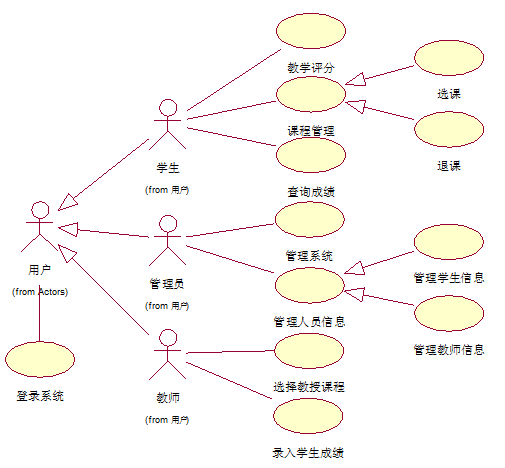
\includegraphics[width=\textwidth]{img/jwxt_usecases.png}
   \caption{教务系统用例析取图}
\end{figure}

\subsection{教务系统用例规约}
\subsubsection{选课用例的用例规约}

\paragraph{简要说明}
  
本用例允许学生注册本学期提供的课程。在学期开始的开放注册时期,学生可以添加或修改选择的课程。课程目录系统提供了当前学期开设的所有课程的列表。
  
\paragraph{事件流}
  \begin{enumerate}
    \item 基本事件流
    
    用例开始于学生选择修改课程表,执行“添加课程”子事件流:
    \begin{enumerate}[(1)]
      \item 系统从课程目录系统中得到课程类别列表(公必、专必、公选、专选),并将列表显示给学生
      \item 学生选择课程类别
      \item 系统从课程目录系统中得到相应课程类别中的课程列表,对列表中的课程检验学生是否满足必要的前置条件,课程是否未被选满且没有时间冲突,然后将满足以上约束的课程列表显示给学生
      \item 学生从课程列表中选择课程
      \item 一旦学生决定了选择某门课程,系统将学生添加到该门课程,用该门课程的课程信息更新课程表,并用“已登记”在课程表中对该门课程进行标记
    \end{enumerate}

    \item 备选事件流
    \begin{enumerate}[(1)]
      \item 不满足前置条件,课程人数已满或课程时间冲突
      
      \CJKindent 如果在添加课程事件流中,系统确定学生没有满足必要的前置条件,或者选择的课程已满,或课程有时间冲突,将显示一条错误信息。学生可选择另一门课程,此用例继续;或取消操作,这时本用例重新开始。
      
      \item 未找到课程表
      
      \CJKindent 如果在增加或删除课程表子事件流中,系统无法返回学生的课程表,将显示错误消息。学生确认错误,这时本用例重新开始。
      
      \item 无法访问课程目录系统
      
      \CJKindent 如果系统无法与课程目录系统取得联系,系统将显示错误消息。学生确认错误,本用例终止。
      
      \item 课程注册系统被关闭
      
      \CJKindent 当用例开始时,如果确定用于本学期的注册系统已被关闭,显示一条消息给学生,本用例终止。学生不能在注册系统关闭后注册课程。
    \end{enumerate}
  \end{enumerate}
  
\paragraph{特殊需求}
  
无
  
\paragraph{前置条件}
  
本用例开始前学生必须已经登陆进系统,且注册员开放注册。
  
\paragraph{后置条件}
  
如果用例成功,学生的课程表被创建,修改,删除。否则系统状态不变。

\begin{figure}[H]
  \centering
  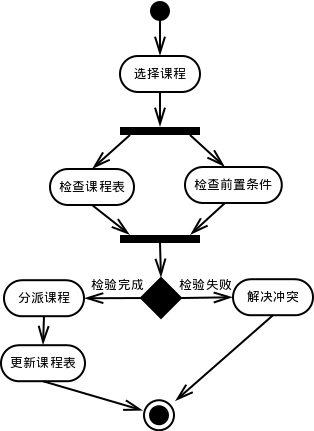
\includegraphics[scale=0.7]{img/jwxt_scourse.png}
  \caption{选课用例过程模型}
\end{figure}

\subsubsection{退课用例的用例规约}
\paragraph{简要说明}
  
本用例允许学生退选除本学期已选择的课程。从学期开始的开放注册时期到学期末的考试阶段前,学生可以退选本学期已选择的课程。
  
\paragraph{事件流}
  \begin{enumerate}
    \item 基本事件流
    
    用例开始于学生选择修改课程表,执行“删除课程”子事件流:
    \begin{enumerate}[(1)]
      \item 系统得到并显示学生当前的课程表
      \item 学生选择要删除的课程,必须选择的课程将不能被选择
      \item 系统检测待删除的课程是否满足必要的预备条件,是否未进入考试阶段,然后提示学生确认删除课程
      \item 学生确认删除
      \item 系统将学生从所选课程中删除,并更新课程表
    \end{enumerate}
    
    \item 备选事件流
    
    \begin{enumerate}[(1)]
      \item 不满足前置条件
      
      \CJKindent 如果在删除课程子事件流中,系统确定学生没有满足前置条件,将显示一条错误信息。学生可选择另一门课程进行删除,此用例继续;或取消操作,这时本用例重新开始。
      
      \item 未找到课程表
      
      \CJKindent 如果在删除课程子事件流中,系统无法返回学生的课程表,将显示错误消息。学生确认错误,这时本用例重新开始。

      \item 无法访问课程目录系统
      
      \CJKindent 如果系统无法与课程目录系统取得联系,系统将显示错误消息。学生确认错误,本用例终止。
      
      \item 选课阶段已结束
      
      \CJKindent 当用例开始时,如果确定本学期的选课阶段已结束,显示一条消息给学生,本用例终止。学生不能在选课阶段结束后退课。
    \end{enumerate}
  \end{enumerate}
  
\paragraph{特殊需求}
  
无。
  
\paragraph{前置条件}
  
本用例开始前学生必须已经登陆进系统,注册员开放注册,且考试阶段未开始。
  
\paragraph{后置条件}
  
如果用例成功,学生的课程表被修改,否则系统状态不变。

\begin{figure}[H]
  \centering
  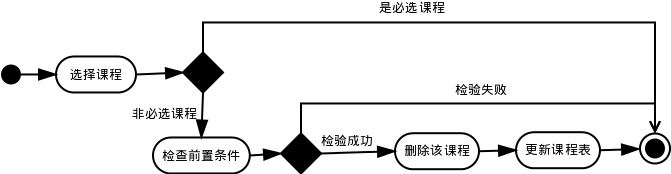
\includegraphics[scale=0.7]{img/jwxt_dcourse.png}
  \caption{退课用例过程模型}
\end{figure}

\subsubsection{教学评分用例的用例规约}

\paragraph{简要说明}
  
本用例允许学生对教师的教学进行教学评分。关闭注册后,学生可以对所选的任意一门课程进行教学评分,期间可以进行修改。在学生查看某一门课程的成绩前,必须先进行教学评分并确认对该门课程教师的教学所作的教学评分,此后教学评分不可修改。
  
\paragraph{事件流}
  
  \begin{enumerate}
    \item 基本事件流
    
    用例开始于学生选择教学评分。
    \begin{enumerate}[(1)]
      \item 系统从课程表中得到学生所选课程,并将未标明“已评教”的课程信息列表显示给学生
      \item 学生从课程信息列表中选择要进行教学评分的课程
      \item 执行“进行教学评分”子事件流
    \end{enumerate}
    
    \begin{enumerate}[{1}.1]
      \item 进行教学评分
      \begin{enumerate}[(1)]
        \item 学生选择对该门课程所评的分数等级,同时可以在文本框中附加说明
        \item 一旦学生确认了教学评分,系统用当前课程的教学评分信息更新教学评分统计
        \item 执行提交教学评分子事件流
      \end{enumerate}
      
      \item 提交教学评分
      
      \CJKindent 系统用“已评教”在课程表中对该门课程进行标记。系统更新并保存课程表。
    \end{enumerate}
    
    \item 备选事件流
    \begin{enumerate}[{2}.1]
      \item 未关闭注册
      
      \CJKindent 提示学生未关闭注册,需要在关闭注册后才能开始教学评分。
    \end{enumerate}
  \end{enumerate}
  
\paragraph{特殊需求}
  
无
  
\paragraph{前置条件}
  
注册员关闭注册。
  
\paragraph{后置条件}
  
如果用例成功,任课老师教学评分信息被更改。否则系统状态不变。

\begin{figure}[H]
  \centering
  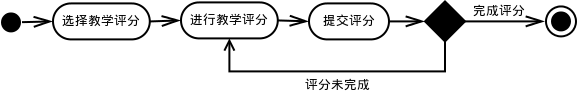
\includegraphics[scale=0.7]{img/jwxt_accessment.png}
  \caption{教学评分用例的过程模型}
\end{figure}

\subsubsection{查询成绩报告用例的用例规约}

\paragraph{简要说明}
  
本用例允许学生查询成绩报告。在查询成绩报告前,必须完成课程的教学评分,否则无法查询成绩报告。
  
\paragraph{事件流}
  
  \begin{enumerate}
    \item 基本事件流
    
    用例开始于学生查询成绩。
    \begin{enumerate}[(1)]
      \item 系统检测学生是否完成教学评分,若已完成则显示学年度、学期、培养类别、课程类别、课程名称(可选)的选项,否则跳转到教学评分页面
      \item 学生选择相应查询选项
      \item 系统返回该学生相应课程的成绩报告并显示
    \end{enumerate}
    
    \item 备选事件流
    \begin{enumerate}[(1)]
      \item 学生未完成教学评分
      
      系统自动跳转到教学评分页面。
      
      \item 导出成绩报告
      
      学生选择要导出的课程,系统将相应的课程成绩以xls格式导出并提供下载。
      
    \end{enumerate}
  \end{enumerate}
  
\paragraph{特殊需求}
  
无。
  
\paragraph{前置条件}
  
学生完成教学评分。
  
\paragraph{后置条件}
  
无

\begin{figure}[H]
  \centering
  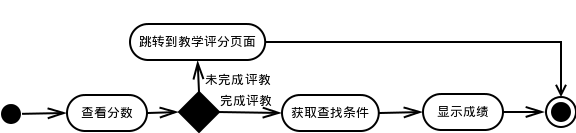
\includegraphics[scale=0.7]{img/jwxt_viewscore.png}
  \caption{查看分数用例的过程模型}
\end{figure}

\subsection{教务系统补充规约}

\subsubsection{目标}
本文档的目的是定义教务系统的需求。本补充规约列出了不便于在用例模型的用例中获取的系统需求。补充规约和用例模型一起记录关于系统的一整套需求。
  
\subsubsection{范围}
  
  \begin{enumerate}
    \item 本补充规约适用于教务系统,将要由学习面向对象软件分析与设计的学生开发。
    \item 本规约除定义了在许多用例中共有的功能性需求以外,还定义了系统的非功能性需求,例如:可靠性、可用性、性能和可支持性等。(功能性需求在用例规约中定义。)
  \end{enumerate}
  
\subsubsection{参考}
无。
  
\subsubsection{功能}
  
  \begin{enumerate}
    \item 多个用户必须能同时执行操作。
    \item 如果某个学生所建的课程表中包含人数已满的课程,必须通知这位学生。
  \end{enumerate}
  
\subsubsection{可行性}
  
用户界面应与IE9/10、Chrome、Firefox、Safari等主流浏览器兼容。
  
\subsubsection{可靠性}
  
教务系统在每周七天,每天二十四小时内都应是可以使用的。宕机的时间应少于10\%。
  
\subsubsection{性能}
  
  \begin{enumerate}
    \item 在任意既定时刻,系统最多可支持2000名用户同时使用中央数据库,并在任意时刻最多可支持500名用户同时使用本地服务器。
    \item 系统将能在十秒钟内提供对课程目录系统数据库的访问。
    \item 注意:基于风险的原型发现课程目录系统数据库在没有利用中层处理能力的前提下,无法满足性能上的需求。
    \item 系统必须能够在2分钟内完成所有事务的80\%。
  \end{enumerate}
  
\subsubsection{可支持性}
  
无。
  
\subsubsection{安全性}
  
  \begin{enumerate}
    \item 系统必须能防止学生修改他人的课程表以及教师修改其他教师所开设的课程。
    \item 只有一门课的教师能输入学生该门课的成绩。
    \item 只有注册员能更改学生的信息。
  \end{enumerate}
  
\subsubsection{设计约束}
  
  \begin{enumerate}
    \item 该系统应与现有课程目录系统(是RDBMS数据库)集成在一起
    \item 系统必须提供可用于各大主流浏览器(IE、Chrome、Safari、Firefox等)的用户接口
  \end{enumerate}

\subsection{术语表}
  \begin{table}[H]
    \caption{术语表}
    \begin{tabularx}{\textwidth}{|l|l|X|l|}
    \hline
    \textbf{术语} & \textbf{英语名称} & \textbf{定义和信息} & \textbf{别名}\\
    \hline
    课程&Course&学生所需学习的科目及其安排&\\
    \hline
    课程表&Schedule&学生所选课程的列表及其详细信息&\\
    \hline
    成绩报告&Score Report&日常考核、期末考试分数、排名等评定的数值&\\
    \hline
    考核方式&Assessment Method&考试的形式,包括提交报告、开卷考试、闭卷考试等&\\
    \hline
    课容量&Capacity&课程可以容纳的学生人数&\\
    \hline
    课程类别&Course Type&课程的分类,包括公共必修课、公共选修课、专业必修课与专业选修课&\\
    \hline
    培养类别&Category&包括主修、辅修、双专业和双学位&\\
    \hline
    教学评分&Evaluation&对教师进行教学评价&评教\\
    \hline
    开课计划&Course Arrangement&课程开设的安排与进度&\\
    \hline
    学籍信息&Student Information&包含学生的个人信息、学习经历&\\
    \hline
    注册&Registration&学生选择课程或老师添加课程信息&\\
    \hline
    退选&Withdrawal&学生取消选择课程&\\
    \hline
    查询成绩&Check Score Report&显示学生的课程成绩、排名、平均绩点&\\
    \hline
    B/S结构&Browser/Server Architecture&Browser/Server 浏览器/服务器结构&\\
    \hline
  \end{tabularx}
  
\end{table}


\subsection{测试用例设计}
\subsubsection{添加课程}
  \begin{itemize}
    \item 前置条件:学生用户选择添加课程选项。
    \item 设计:
    \item 步骤——系统从课程目录系统中得到可选择的课程列表,并将列表显示给学生。
    \item 检验点——课程列表正确地被显示。
    \item 步骤——显示空白课程表并提示学生选择四门主要课程和两门备选课程;
    \item 检验点——空白课程表被正确地显示。
    \item 步骤——如果学生选择相应课程并提交。
    \item 检验点——如果课程选择符合条件,则所选课程标记为已登记。
    \item 检验点——系统正确地保存了课程表。
    \item 检验点——在课程人数已满,有时间冲突,课程数量不符的异常情况下,系统是否做出预期的反应。
    \item 步骤——如果学生选择相应课程并保存。
    \item 检验点——所选课程标记为已选。
    \item 检验点——系统正确地保存了课程表。
    \item 后置条件:成功测试该用例后,确保退出注册课程。
    \item 可接受标准:所有的检验点必须成功。
  \end{itemize}


% 教务系统设计
\newpage
\begin{center}
  \section{教务系统设计}
\end{center}

\subsection{系统框架}\label{sec:system_frame}
本系统基于层次化、模块化的思想进行搭建和开发。系统分为三层,分别为:表示层,控制层以及实体层。该三层分层结构具有明晰的依赖关系,表示层依赖于控制层,控制层调用实体层,如图\ref{fig:level_depend}所示。本文使用包图的形式描述系统各层各模块的依赖关系,如图\ref{fig:system_arch}所示。

\subsubsection{表示层}
  
表示层是用户与系统交互的界面,负责获取用户的请求和信息,展示系统的操作结果给用户。本系统表示层的边界类包括

\begin{itemize}
  \item 登录认证(~\texttt{Login}~)
  \item 学生选课退课(~\texttt{StudentGetCourse}~)
  \item 学生教学计划(~\texttt{StudentGetPlan}~)
  \item 学生查看课表(~\texttt{StudentGetSchedule}~)
  \item 学生教学评分(~\texttt{StudentGetAssessment}~)
  \item 学生成绩报告(~\texttt{StudentGetScore}~)
  \item 教师开课计划(~\texttt{TeacherGetPlan}~)
  \item 教师成绩管理(~\texttt{TeacherManageScore}~)
  \item 管理员学籍管理(~\texttt{AdministratorManageSchoolroll}~)
  \item 管理员教籍管理(~\texttt{AdministratorManageTeacherpost}~)
  \item 管理员查看评教(~\texttt{AdministratorViewAssessment}~)
  \item 管理员课程管理(~\texttt{AdministratorManageCourse}~)
  \item 管理员成绩管理(~\texttt{AdministratorManageScore}~)
\end{itemize}
  
\subsubsection{控制层}
  
控制层是系统业务逻辑的核心,控制管理系统的运行。它负责接收用户的请求和信息,调用实体层的数据,执行系统的业务逻辑操作,并最终将操作结果返回给用户。本系统控制层的控制类包括:
\begin{itemize}
  \item 用户管理(~\texttt{user.views}~)
  \item 学生管理(~\texttt{student.views}~)
  \item 老师管理(~\texttt{teacher.views}~)
  \item 管理员管理(~\texttt{administrator.views}~)
  \item 课程管理(~\texttt{course.views}~)  
  \item 评教管理(~\texttt{assessment.views}~)
  \item 选课信息管理(~\texttt{take.views}~)
  \item 学院信息管理(~\texttt{school.views}~)
  \item 界面渲染控制类(~\texttt{EduAdminSystem.views}~)
\end{itemize}
  
\subsubsection{实体层}
  
实体层是系统的数据实体层,在实体层与控制层之间是数据访问对象层(DAO),DAO层提供了控制层访问实体层的接口方法。本系统实体层的模块(实体类)包括:
\begin{itemize}
  \item 学院信息(~\texttt{School, Department, Speciality, Class}~
  \item 课程信息(~\texttt{Course, CourseTime}~)
  \item 选课信息(~\texttt{Take}~)
  \item 教学评分信息(~\texttt{Assessment}~)
  \item 用户信息(~\texttt{User, Administrator, Teacher, Student, StudentMeta, Permission}~)
  \item 全局状态信息(~\texttt{GlobalData}~)
\end{itemize}

\begin{figure}[H]
  \centering
  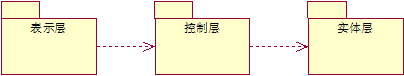
\includegraphics[width=0.8\textwidth]{img/level_depend}
  \caption{层依赖关系}
  \label{fig:level_depend}
\end{figure}

\begin{figure}[H]
  \centering
  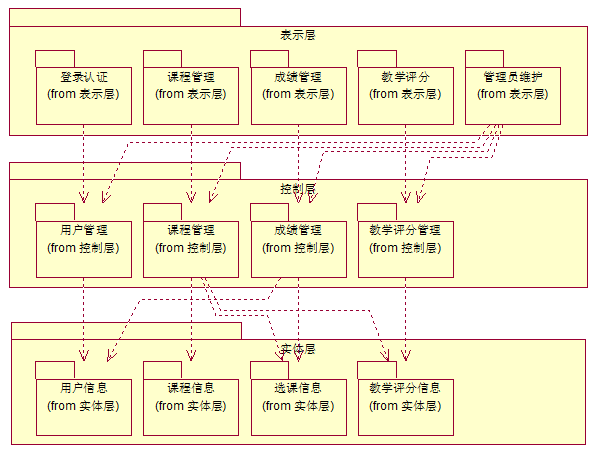
\includegraphics[width=\textwidth]{img/jwxt_system_arch}
  \caption{系统框架图}
  \label{fig:system_arch}
\end{figure}

\subsection{系统关键抽象}\label{sec:system_key_abstract}
系统关键抽象即系统实体类图,系统实体类图描述了系统中的类及其相互之间的关系,它反映了系统中包含的各种对象的类型以及对象间的各种静态关系。图\ref{fig:system_entity}是对实体层中各模块的细化,主要描述了系统实体层中各实体类的属性及其相互的关系。

\begin{figure}[H]
  \centering
  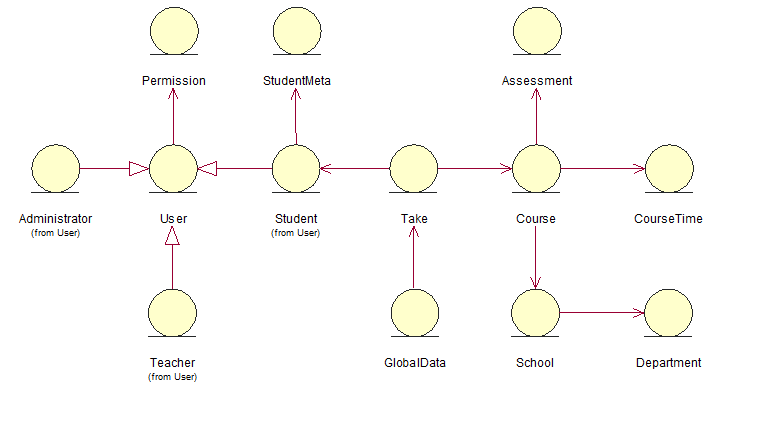
\includegraphics[width=0.95\textwidth]{img/system_entity}
  \caption{系统实体类图}
  \label{fig:system_entity}
\end{figure}
\subsection{用例分析}
\subsubsection{分析类及其功能}
由于系统的用例较多,难以一一列举,所以选取“选课”和“查询成绩”两个用例进行详细分析。其它的用例分析与此两例相似。每个用例分析由四部分组成,第1部分用例功能描述,对用例功能进行简单的描述,第2部分用例交互过程,主要描述了用户与系统的交互工程,采用时序图进行描述,第3部分用例的类分析和实现,描述了用例涉及的各种类,包括边界类,控制类和实体类,第4部分分析类关联关系,描述了分析类的关联关系。

\paragraph{选课用例分析}
\subparagraph{选课用例功能描述}
学生可以利用本功能注册当前学期提供的课程。

\subparagraph{选课用例交互过程}
    
该用例始于学生使用“选课”功能。
    
\begin{enumerate}
  \item 系统将课程类别列表(公必、专必、公选、专选、体育课)显示给学生;
  \item 学生选择课程类别;
  \item 系统从课程目录系统中得到相应课程类别中的课程列表,对列表中的课程检验学生是否满足必要的前置条件,课程是否未被选满且没有时间冲突,然后将满足以上约束的课程列表显示给学生;
  \item 学生从课程列表中选择课程;
  \item 一旦学生决定了选择某门课程,系统将学生添加到该门课程,用该门课程的课程信息更新课程表,并用“已登记”在课程表中对该门课程进行标记。
\end{enumerate}
    
图\ref{fig:selectcourse_secquence}是选课用例的时序图
\begin{figure}[htbp]
  \centering
  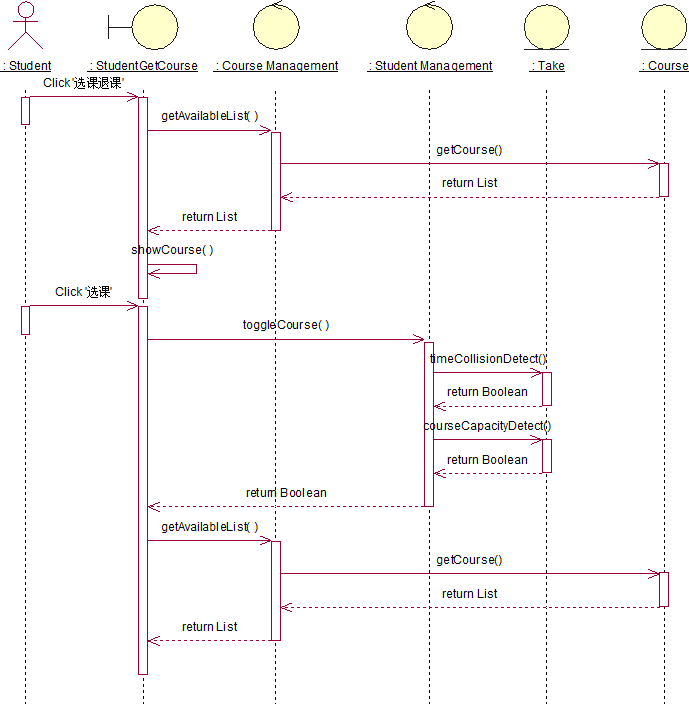
\includegraphics[width=0.7\textwidth]{img/selectcourse_secquence}
  \caption{选课用例时序图}
  \label{fig:selectcourse_secquence}
\end{figure}
    
\subparagraph{选课用例的类分析与设计}
\begin{itemize}
  \item 边界类:课程列表界面(~\texttt{StudentGetCourse}~)。该界面的组件主要用于显示该学生本学期可选课程,以及获取学生的选课请求。

  \item 控制类:课程管理(~\texttt{CourseManager}~)。调用~\texttt{getTakes()}~方法获取已选课信息,调用\texttt{getCourses()}获取可选课程信息。获取学生选课请求之后,调用~\texttt{checkCollision()}~\\检测待选课程是否与已选课程存在冲突;若无冲突,则调用~\texttt{take()}~把选课课程加入到选课信息表中;最后再调用~\texttt{getTakes()}~和~\texttt{getCourses()}~更新已选课程列表和可选课程列表。

  \item 实体类:实体类有两个,分别为选课信息(~\texttt{Take}~)和课程信息(~\texttt{Course}~)。前者存储了学生选课的各种信息,包括选课课程信息、学生信息、课程成绩等;后者存储课程信息,包括课程名、开课院系、老师名、开课时间、学分、考查方式、课程类别、教学评分平均成绩及已进行教学评分的人数等等。
\end{itemize}
    
\subparagraph{选课用例分析类关联关系}
由选课用例的交互过程,可得选课用例分析类关联关系如下:
\begin{figure}[H]
  \centering
  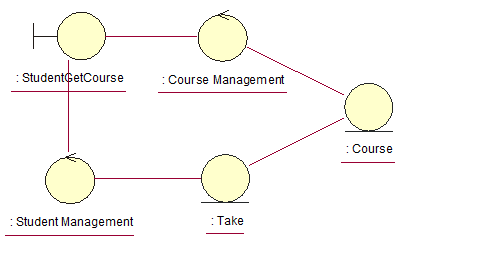
\includegraphics[width=\textwidth]{img/selectcourse_depend}
  \caption{选课用例分析类关联关系图}
\end{figure}
  
\paragraph{查询成绩用例分析}
\subparagraph{查询成绩用例功能描述}

学生可以利用本功能查询个人已选课程的成绩。
    
\subparagraph{查询成绩用例交互过程}
    
该用例始于学生使用“查询成绩”功能。
\begin{enumerate}
  \item 系统显示学年、学期、培养类别等选项;
  \item 学生选择相应查询选项;
  \item 系统检测学生是否完成教学评分,若已完成则返回该学生相应课程的成绩报告并显示,否则给出未评教课程的列表。
\end{enumerate}
    
图\ref{fig:query_achievement_sequence}是查询成绩用例的时序图
\begin{figure}
  \centering
  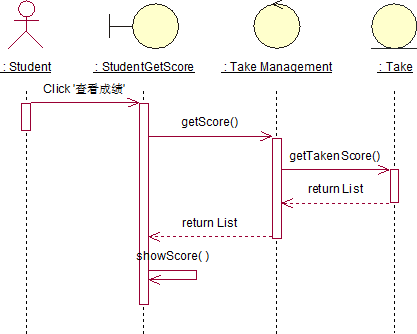
\includegraphics[width=0.7\textwidth]{img/query_achievement_sequence}
  \caption{查询成绩用例时序图}
  \label{fig:query_achievement_sequence}
\end{figure}
    
\subparagraph{查询成绩用例的类分析与设计}
\begin{itemize}
  \item 边界类:查询成绩界面(~\texttt{StudentGetScore}~)。该界面的组件主要用于获取学生查询某学期成绩的请求,并显示该学生相应学期的课程成绩。
  \item 控制类:成绩管理(~\texttt{ScoreManager}~)。当获取学生查询某学期成绩的请求之后,调用~\texttt{getTakes()}~取得该学生相应学期的选课列表信息。通过该列表的条目,先判断该学生是否完成教学评分。若无,则跳转至教学评分界面;否则提取条目中的成绩信息,并调用~\texttt{getCourses()}~获取该课程名称、学分等信息,最后将这些信息一并显示到查询成绩界面中。
  \item 实体类:实体类有两个,分别为选课信息(~\texttt{Take}~)和课程信息(~\texttt{Course}~)。前者存储了学生选课的各种信息,包括选课课程信息、学生信息、课程成绩等;后者存储课程信息,包括课程名、开课院系、老师名、开课时间、学分、考查方式、课程类别、教学评分平均成绩及已进行教学评分的人数等等。
\end{itemize}
    
\subparagraph{查询成绩用例分析类关联关系}
由查询成绩用例的交互过程,可得查询成绩用例分析类关联关系如下:
\begin{figure}[H]
  \centering
  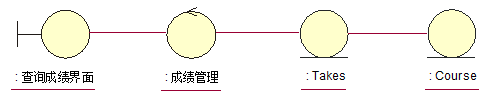
\includegraphics[width=\textwidth]{img/query_achievement_depend}
  \caption{查询成绩用例分析类关联关系图}
\end{figure}

\subsubsection{分析类到分析机制映射}
由于系统的用例较多,难以一一列举分析类到分析机制映射,因此只针对查询成绩用例进行分析类到分析机制映射。涉及的分析类有选课信息类(~\texttt{Take}~),课程信息类(~\texttt{Course}~),成绩管理类(~\texttt{ScoreController}~)。分析类到分析机制的映射如表\ref{table:anaClass_to_anaMechanism}所示。

\begin{table}[H]
  \caption{部分分析类到分析机制映射表}
  \label{table:anaClass_to_anaMechanism}
  \begin{tabularx}{\textwidth}{|Y|Y|}
  \hline
  \textbf{分析类}&\textbf{分析机制}\\
  \hline
  选课信息&永久性、安全性\\
  \hline
  课程信息&永久性、安全性\\
  \hline
  成绩管理&分布式、安全性\\
  \hline
  \end{tabularx}
\end{table}
\subsubsection{系统类图}
由系统关键抽象,设计各实体类的详细成员,得系统类图,如图\ref{fig:system_class}所示。
\begin{figure}[htbp]
  \centering
  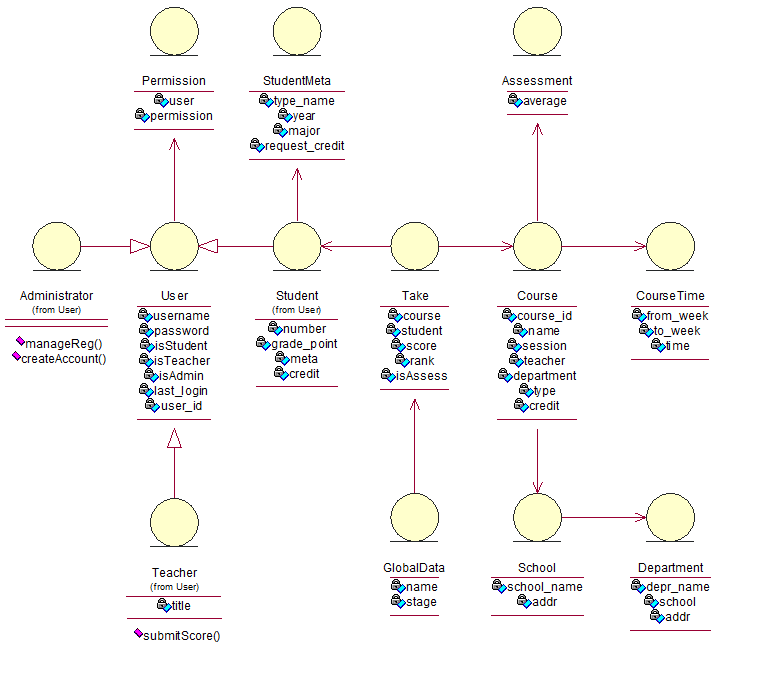
\includegraphics[width=0.95\textwidth]{img/system_class}
  \caption{系统类图}
  \label{fig:system_class}
\end{figure}


% 附录
\newpage
\appendix
\begin{center}
  \section{人员职责与分工}
\end{center}

\begin{itemize}
  \item 叶晓军:组长,主要负责项目人员组织、进度管理、系统业务逻辑设计
  \item 杨曦华:主要负责系统前端设计
  \item 柯毅豪:主要负责系统后台设计、系统部署
  \item 钟宇腾:主要负责系统架构设计、代码管理
  \item 系统测试与性能调优由全体成员共同完成。
\end{itemize}


\newpage

\begin{center}
  \section{项目开发使用的技术说明}
\end{center}

\subsection{系统架构}
\begin{itemize}
  \item Django Web~框架(项目主页:https://www.djangoproject.com/)
  
  \CJKindent 本系统基于~django web~框架进行开发。~Django Web~框架是一个高级~Python\footnotemark[1] Web~框架,提供~ORM (~Object-relational mapper)~方法,可以完全使用~Python~来定义数据库的表及其元素,并封装了大量的数据库访问~API~,把数据库元素映射为~Python~内部类型,兼容多种数据库后台;提供~Template~系统,可以在~HTML~中嵌入~Python~代码便于服务器动态生成页面;提供缓存模块,提高服务器运行效率。
  
  \item Bootstrap前端框架与交互组件集(项目主页:http://twitter.github.com/bootstrap/)
  
  \CJKindent 本系统前端基于~Bootstrap~模板进行开发。~Bootstrap~是用于快速开发~Web~应用的前端工具包。它是一个~HTML, CSS, JavaScript~的集合,它使用了最新的浏览器技术,给~Web~开发提供了时尚的版式、表单、按钮、表格、网格系统等等。
  
  \item PostgreSQL数据库
  
  \CJKindent 我们的项目使用~PostgreSQL~数据库作为数据库后台,~PostgreSQL~是自由的对象-关系数据库服务器(数据库管理系统),在灵活的~BSD~许可证下发行。~PostgreSQL~使用~SQL~语言来在执行资料的查询。这些资料通过连外键联系在一起,以一系列表格的形式存在。~PostgreSQL~相对于竞争者的主要优势,主要的特征为可编程性:对于使用数据库资料的实际应用,~PostgreSQL~让开发与使用的工作,变得更加容易。与PostgreSQl配合的开源软件很多,有很多分布式集群软件,如pgpool、pgcluster、slony、plploxy等等,很容易做读写分离、负载均衡、数据水平拆分等方案。
  
  \CJKindent 教务系统经常需要处理高并发情形,~PostgreSQL~是多进程的,在并发不高时处理速度略慢于~MySQL~等多线程数据库,但当并发高的时候,对于现在多核的单台机器上,~PostgreSQL~能利用多核处理器的并发处理优势,整体性能优于其它基于多线程的数据库。
\end{itemize}

本系统是一个基于~Web 2.0~架构的系统,前端使用~AJAX (Asynchronous JavaScript and XML)~来动态显示内容和响应用户输入,服务器采用~Django~网络框架处理数据。在处理请求时不返回整个网页而是只返回用~JSON (Javascript Object Notation)~表示的数据,前端框架处理数据并呈现,不刷新整个页面而只更新页面的部分内容。

采用此架构可以节约网格资源,在服务器处理大量情求时(如选课时期),可以节约服务器资源和网络带宽,提高网站的响应速度,减轻服务器负担。

本系统在设计时充分考虑到跨平台的需要,兼容绝大多数主流的浏览器(包含桌面系统与手持设备系统的浏览器),在呈现时自动检测显示区域分辨率,若检测到是手持设备的分辨率,则会显示一个专门优化过的页面,提升用户体验。

\footnotetext[1]{Python~是一种面向对象的解析性编程语言、动态语言,支持命令式程序设计、面向对象程序设计、函数式编程、面向切面编程、泛型编程多种编程范式,具备垃圾回收功能,能够自动管理储存器使用。语言设计的哲学是“用一种方法,最好是只有一种方法来做一件事”,语法简洁少有岐义,代码可读性高。}

\subsection{代码托管与版本控制}
\begin{itemize}
  \item Git~版本控制系统
  
  \CJKindent Git~是一个由~Linus Benedict Torvalds~为了更好地管理~Linux~内核开发而创立的分布式版本控制/软件配置管理软件。与常用的版本控制工具~CVS、Subversion~等不同,它使用了分布式版本库,不需要服务器端软件支持,使源代码的发布和交流极其方便。~Git~的速度很快,这对于诸如~Linux kernel~这样的大项目来说自然很重要。~Git~最为出色的是它的合并跟踪(~merge tracing~)能力。
  
  \item GitHub
  
  \CJKindent GitHub~是一个基于互联网、使用~Git~版本控制系统的项目存取服务,提供了诸如~feeds~,~followers~,开发者的工作网络图表等统计服务。根据在2009年的~Git~用户调查,~GitHub~是最流行的~Git~存取站点。
  
  \CJKindent 我们的项目托管于~GitHub~,地址为~https://github.com/zonyitoo/SYSUEduAdminSystem~,使用~Git~版本控制系统来进行版本控制和软件配置管理。
\end{itemize}

\newpage
\begin{center}
  \section{开发总结与心得感悟}
\end{center}

\subsection{版本控制系统图表分析}
\begin{figure}[H]
   \centering 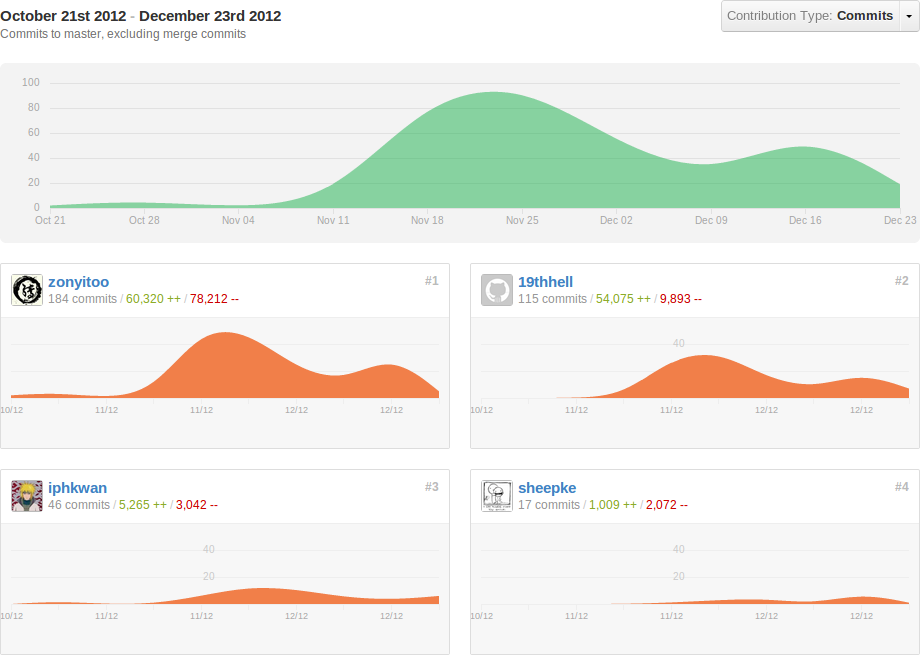
\includegraphics[width=\textwidth]{img/contrib.png}
   \caption{项目成员贡献及项目提交数与时间关系图}
\end{figure}

上图中,帐号与成员的对应关系为:钟宇腾(~zonyitoo~)、杨曦华(~19thhell~)、叶晓军(~iphkwan~)、柯毅豪(~sheepke~)。我们的项目从2012年10月21日开始编写,至2012年12月23日完成。在2012年11月20日前后进行基础框架搭建,并推出~Alpha~测试版,在2012年12月16日前后对于系统细节修补及加入新功能,推出~Beta~测试版。

钟宇腾(~zonyitoo~)是项目代码的管理员,主要负责项目文件树管理及架构设计,因此提交数(~Commits~)最多,增加了60320行代码,删除78212行代码;杨曦华(~19thhell~)是网页前端开发者,主要负责网页前端设计,有115次提交,增加了54075行代码,删除9893行代码;叶晓军(~iphkwan~)是组长,主要负责项目进度管理,有46次提交,增加5256行代码,删除3042行代码;柯毅豪(~sheepke~)是系统后台开发者,主要负责后台服务器响应代码编写及服务器维护及测试,有17次提交,增加1009行代码,删除2072行代码。全组所有成员在基本分工下互相合作,并没有很绝对的分工界线。

\begin{figure}[H]
   \centering 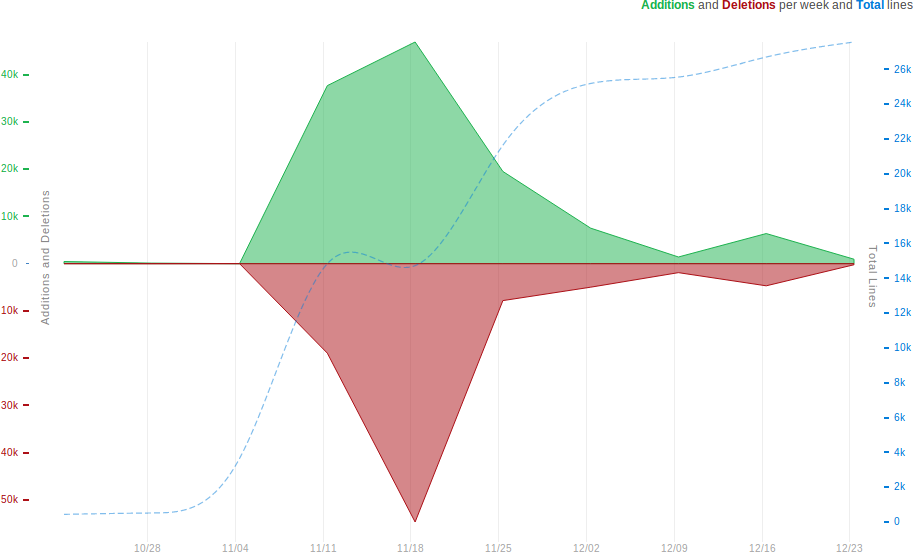
\includegraphics[width=\textwidth]{img/code_freq.png}
   \caption{项目代码变化图}
\end{figure}

图中虚线是代表代码行数的变化与时间的关系,2012年12月23日后代码行数超过了2.6万。中央横线以上的图中,高度代表该时间段增加的代码行数;中央横线以下的图中,高度代表该时间段被删除的代码行数,总体体现了代码增加的速度。\vspace{2em}

项目托管主页:https://github.com/zonyitoo/SYSUEduAdminSystem

项目统计图:https://github.com/zonyitoo/SYSUEduAdminSystem/graphs

\subsection{个人总结与感悟}
\begin{itemize}
  \item 叶晓军
  
  \CJKindent 本学期初,本人联系上杨曦华、柯毅豪和钟宇腾三位编程牛人组队,并十分荣幸地被推举为组长,开始了软件工程课程项目的设计与开发。作为项目的负责人,在项目中我更多地负责人员的组织与开发进度的管理。
  
  \CJKindent 在项目开发过程中,我遇到的第一个挑战就是,我和小组各成员都不甚了解网站开发技术。因此,在项目起步阶段,如何确定网站的开发框架、合理地分工学习网站开发技术变得十分重要。在与小组成员的多次讨论交流中,我大致了解到,杨曦华擅长图像的设计与处理;柯毅豪对系统后台有一定的认识,擅长系统的部署;钟宇腾热衷于追求最新的技术,拥有敏锐的技术触觉;而至于我自己,大学前两年的ACM/ICPC锻炼经历让我具备了不错的逻辑分析设计能力与代码查错能力。由于小组中我和钟宇腾之前已熟悉Python语言,为了降低学习成本,我们敲定了网站后台使用由Python语言开发的、当前业界新兴起来的Django框架,由柯毅豪和钟宇腾负责。同时,擅长页面设计的样曦华毫无疑问地负责网站前端的设计,开始了html/css/ajax等相关网页设计技术的深入学习。为了沟通好前后端,虽不深入,但作为组长的我必须对所有技术都有所涉猎,在开发中后期主力负责代码的查错调优。
  
  \CJKindent 作为一个项目团队,成员间的沟通协作非常重要。如果我们四人分别在各自的地方进行编码,利用qq、gmail等网络通讯工具进行交流协作,效率将十分低下。因此,我选择了四人都空余的每周周五下午,到学院楼的学术讨论室,集中进行项目核心功能代码的编写。集中编码的另一个好处就是,通过聆听小组成员的技术讲解,我们可以更加高效地学习自己之前不熟悉的技术。此外,技术讲解也是一个锻炼自己表达能力的过程,在讲解讨论中,讲解人也能加深对技术的认识,整个项目的编码质量也会得到提高。
  
  \CJKindent 回顾整个软件工程过程,从立项、文档编写,到代码开发、调试部署,我受益匪浅。在文档编写阶段,我体会到文档格式严谨的重要性,通过对图表、文字表述的反复修改,我提高了文字表述能力;在代码开发阶段,我学习了许多前沿的网站开发技术,这对我日后个人职业发展具有深远影响;在代码查错调优阶段,我体会到工程代码与ACM编程比赛的编码的不同,工程编码需要程序员更加注重代码的可读性与可维护性……最后,衷心感谢衣杨老师对我、对我们小组项目的指导和帮助,您给我们指出的不足让我们看到了自己发展的潜力;感谢三位给力的队友对本人工作的支持和配合,能在融洽的团队开发氛围下互相学习、一起工作是一种美妙的享受。
  
  \item 杨曦华
  
  \CJKindent Todo.
  
  \item 柯毅豪
  
  \CJKindent 在学习软件工程之前,我编写的程序大多数都是算法和数据交织在一起,尽管后来将数据独立出来保存在文件中,不过为了处理输入输出的格式问题,依旧需要浪费很多时间。在学习了MVC架构之后,更加能够理解数据库系统在大型软件项目中的重要性。
  
  \CJKindent 在这个学期编写教务系统这个项目的过程中,我学到了很多不同方面的东西。以前写程序时,不会先编写文档,而是直接开始构思代码,虽然看起来节省了时间,不过到了中间就会发现原来的构思有缺陷,需要推倒重来。而通过小组成员间讨论软件架构的组成,然后再一步一步抽象出各个类,这种方法使得后面的实现过程更加顺畅,也降低了重构发生的可能性。
  
  \CJKindent 在实现教务系统的过程中,小组决定使用Python语言和Django框架。我之前并没有接触过Python语言和Django框架。不过在浏览了相关的Python书籍和Django手册后,再结合小组成员已有的代码,我也能够做到边学边用,逐渐完成了选课退课和课程筛选部分的后台代码编写工作。这三个月的过程让我感受到,已有多少知识和技能并不是最重要的,关键是有足够的学习能力,在给定的时间内学会并应用新的知识。
  
  \CJKindent 软件工程项目和之前个人的小项目相比,更注重团队合作。这次项目是我第一次依赖Git和Github进行代码的版本管理。团队中的每一个人提交了代码之后,如果备注了哪个地方存在bug,大家很快就会互相讨论如何解决,而不是仅靠一个人的力量苦苦挣扎。这种团队合作的氛围使得工作的效率大大提升。
  
  \item 钟宇腾
  
  \CJKindent 在本次软件工程的项目小组中,我主要负责架构设计、项目管理、服务器后台软件编写。
  
  \CJKindent 我们小组的成员都喜欢尝试新技术,比如在编写分析与设计文档时,我们为了让大家都更方便地参与到文档的编写中去,采用了在线文档协作平台—— Google Docs进行文档的编写,可以多人同时在线对一个文档的各个不同部分进行编写,提高了工作效率,在自己编写文档的同时也能让其它组员检查错误,提高文档的质量;在代码编写时,我们使用了版本控制工具,使得每个成员都能及时得到最新的代码,及时发现和修正错误,出现重大错误时可以方便回滚到历史上某个正常版本,有利于迭代开发,提高编码效率和软件质量;我们的所有代码都托管到网站上,所有成员都可以对某一次的提交留言,方便成员间交流合作;还有全新的数据库后台系统、全新的编程语言……得益于使用当前比较流行的新技术,使我们能够在两个半月的时间里顺利完成项目的开发与测试工作,采用开源技术使我们从开源社区中获益良多。
  
  \CJKindent 在本次软件项目开发过程中,我收获最大的是体验团队合作的氛围。在合作过程中,成员间出现的各种分歧是影响开发进度和团队凝聚力的重要因素,沟通是解决分歧的重要手段。通过互相沟通,理解对方的立场,团队成员相互磨合,最后得出大家都满意的结果。在讨论中的思维碰撞也有利于得出更优的解决方案,有利于提高软件质量。
  
  \CJKindent 通过本次软件工程的项目,我在学习到许多的新技术之余,更大的收获是团队的合作经验。新技术有利于我了解当今时代信息技术的发展方向以及掌握更多更有用的技术,团队合作的经验则有利于我未来真正加入到团队中时更好的融入团队、发挥自己的能力。因此本次项目实践于我来说是一次非常宝贵的经验,感谢衣杨老师及我的队友。

\end{itemize}


\newpage
\end{CJK*}
\end{document}
